%% ----------------------------------------------------------------------------
% BIWI SA/MA thesis template
%
% Created 09/29/2006 by Andreas Ess
% Extended 13/02/2009 by Jan Lesniak - jlesniak@vision.ee.ethz.ch
%% ----------------------------------------------------------------------------
\newpage
\chapter{Materials and Methods}

This project consists of two parts. When given a set of photos taken using a
mobile phone, the first part is the selection of photos and the second part is
the cropping of photos.
The selection criteria is wallpaper suitability while the cropping aims to
retain interesting areas to result in a well composed final image.

Both decisions are subjective by nature.
If a set of rules were defined to make the decisions, the process would
inherently be biased, and results difficult to evaluate.
Thus for both selection and cropping, machine learning is utilised with aims to
avoid introducing unnecessary bias.


\section{Selection\label{sec:meth_selection}}

When considering a single photo, whether this photo could be used as a wallpaper is a subjective decision.
Ultimately, the decision depends on whether a photo is aesthetically pleasing to view in the background of the home screen of a mobile device.
This may depend not only on the objects present in the scene, but image sharpness, colour composition, and density of detail.
At the most basic level, it can be argued that the most important factor is the objects present.
For instance, person A may prefer having city skylines on their wallpapers, while person B may prefer distant mountain peaks.
When considering objects which most people would not like to have on their wallpapers, we can think of posters, advertisements, and price tags as examples.
The detection of such objects would allow for a simple but effective way of picking or discarding images when attempting to find a suitable wallpaper.
We therefore suggest a simple algorithm which performs object class recognition to determine if an image is suitable as a wallpaper.

To address the inherent subjectivity of this process, we employ machine learning and acquire annotations from multiple individuals.
By doing so, it is possible to train a model such that it can cater to the preferences of all annotators as well as possible.
A feature vector is created per image, encoding information on detected objects.
These vectors can be used to train a SVM.

One way of performing object class recognition is via the use of deep
convolutional neural networks.
An existing implementation is one provided by Caffe, a deep learning framework\cite{jia2014caffe}.
Caffe provides several models trained for the ILSVRC 2012 dataset \cite{ILSVRC15}.
This dataset consists of 150,000 photographs and 1,000 associated object classes.

In a deep convolutional neural network, different convolutions are performed at
each neuron with a focus on different portions of a given image.
In \cite{DonahueJVHZTD13}, it is determined that using the activations of the
hidden fully connected layer, \texttt{fc7} in conjunction with a SVM results
yields the best classification results in domain adaptation tasks such as scene recognition.


Therefore, an input image is propagated through the trained neural network and
the activations at hidden layer \texttt{fc7} is used as the given image’s
representative feature vector.
The exact neural network used is \texttt{bvlc\_reference\_caffenet}.
This results in 4096 features per image.
These feature vectors are used to train a SVM.
The decision function of the trained model calculates a suitability score when
provided a feature vector representative of an input image.
If an image is classified as positive, it is considered to be suitable.

The resulting model can then be used to classify new images.
Figure \ref{fig:pipeline_selection} shows the full pipeline for
checking the suitability of an image as a wallpaper on a mobile device.

\begin{figure}
\centering\includegraphics[width=0.7\columnwidth]{../figures/pipeline_suitability.pdf}
\caption{Full pipeline for determining if an image is suitable for use as a wallpaper.\label{fig:pipeline_selection}}
\end{figure}

This portion of the project is implemented using \texttt{Python},
\texttt{scikit-learn}, \texttt{OpenCV}, and \texttt{PIL}.

\subsection{Datasets}

Two datasets were created for the selection step. I will call these datasets the
\emph Michael dataset and the \emph Wookie dataset.

The Michael and Wookie datasets consist of 275 and 266 images each respectively.
The photos image a variety of objects and scenes with some example objects
as listed below:

\begin{itemize}
\item Natural landscapes (Mountains, rivers)
\item Man-made landscapes (Cityscapes, landmarks)
\item Text (Poster, presentation, street sign)
\item Dim indoors (Concert, restaurant, presentation)
\end{itemize}

While the photo collections were created with aims to provide sufficient variety
to result in a more general purpose model, privacy was respected and thus the
datasets lack people.

The ground truth was collected by annotation from 4 different volunteers.
Each person was asked to mark images in both datasets as either suitable or
unsuitable (1 or 0 respectively) based on the simple rule: \emph{"rate as
suitable if you would personally use the image or a portion of the image as a
wallpaper on your phone"}.

In early annotations, it was evident that the order in which images was
displayed affected final decisions.
If similar images were shown in succession, the classifications could become
less consistent.
The order was therefore randomised.
A simple Python script was written to accommodate this effort.
Key bindings were added to allow for effortless annotation and navigation
between images, and the images are tinted green or red depending on the decision
to allow for quick review.

A further improvement could be made by splitting annotators into two groups, one
which make a preliminary set of annotations which can be used to create a
balanced dataset which is annotated by the other group of annotators.
This would reduce bias further.

\section{Cropping\label{sec:method_cropping}}

This study bases its cropping method on \cite{fang2014automatic} with modifications.
The differences are namely in moving boundary simplicity into the learning phase, the use of shrinking crop region candidates in crop selection, and the use of a Reddit based dataset.
This is further outlined below as the algorithm is explained.

To crop an image automatically, it should be possible to find out which regions
of the image are worth retaining.
To do so, we consider visual saliency.
Visual saliency is a measure which represents how distinct a region is in
relation to its neighbouring regions \cite{borji2013state}.
Many saliency map algorithms have been suggested in the past, with ground truth
collected by tracking the eye movements of human participants.

The algorithm selected for generating visual saliency maps is the boolean map
based approach or BMS \cite{zhang2013saliency}.
This approach randomly thresholds each channel in CIE Lab colour space to
generate a set of boolean maps, then averages the boolean maps to generate an
attention map.
The algorithm is very fast and produces high quality saliency maps.
The output saliency map is further dilated and blurred in an attempt to give
crop candidates a good margin from objects.

An input image is first scaled to be at most 800 pixels wide or high, then a
dilation width of $2$ pixels and step size of $6$ is used to generate an initial
saliency map.
This map is further processed with a dilation filter of width $5$ pixels and a
$11\times11$ gaussian blur filter with $\sigma=50$.

In \cite{fang2014automatic} automatic cropping is done using three distinct metrics.
These are saliency composition, boundary simplicity, and content preservation.
Saliency composition concerns the layout of saliency energy, and boundary
simplicity is whether the crop cuts through objects, while content preservation
is the proportion of saliency energy kept in the crop.
In our approach saliency composition and boundary simplicity are encoded into
the learning stage where an SVM is trained to distinguish between well and badly
composed images or crops.
The content preservation metric is used in the filtering of crop candidates in
the cropping stage.

Saliency composition is represented by a 4-level spatial pyramid of the saliency
map.
This is done by resizing the map into $8\times8$, $4\times4$, $2\times2$, and
$1\times1$ patches
by averaging pixel values, then using pixel values in these patches as features.
This results in 85 features which encode the distribution of saliency energy.

Boundary simplicity aims to encourage crops which do not cut through objects.
This can be done by taking a gradient map of the original image.
A 2-pixel wide strip is taken for each edge and the mean value is used as a
feature.
This results in 4 features encoding the amount of edges crossed by a given
crop's boundary.
This is different from the implementation in \cite{fang2014automatic} where a single boundary simplicity score is used later on in the evaluation of candidate crop regions.
We introduce these changes for two reasons.
The first is to avoid the weighting issue when dealing with multiple metrics in the final scoring of crop candidates, instead relying on SVM.
The second reason is to allow for boundary metric to adapt to cases where saliency composition may affect boundary values.
For example, a portrait photo of a person may have high saliency on the bottom edge of the image but still be considered to be well composed with good boundary simplicity.

The gradient map of an image is created by first resizing the image to be at
most 600 pixels wide or high, then applying a first-derivative $5\times5$ Sobel
filter.
Absolute values are taken per pixel, then a $11\times11$ Gaussian blur filter
($\sigma=50$) is applied.
This results in an image similar to the corresponding saliency map where object
boundaries are blurred to encourage good margins in crop candidates.

When considering saliency composition and boundary simplicity, the final number
of features used to represent an image is 89.
These features are used to train a SVM.
The method of annotating crops as well or badly composed is outlined in section
\ref{sec:Cropping_Dataset}.
The SVM trained is C-SVC with a linear kernel where 20-fold cross-validation is
used to find the hyperparameter $C$.

The trained model can be used to assign a score to a candidate crop. For any
given image, thousands of crop candidates are generated and evaluated to find
the best crop.
Specifically, $4000$ initial crop candidates are generated, and a content
preservation score ($S_{content}$) is evaluated.
The score as given by equation \ref{eq:S_content} represents how much
interesting information is retained by the suggested crop.
By using this score, one can discard inappropriate crops early on without
comparing scores given by the trained model.
Crops above a threshold score are retained in a list of crop candidates.
The threshold is reduced until a target number of crops is reached.
This algorithm is described in algorithm \ref{alg:autocrop}.

\begin{algorithm}
\begin{algorithmic}[1]

\State $saliency \gets$ Saliency Map
\State $thresh \gets 0.7$
\State $n \gets 0$
    \Repeat
    \State Generate $4000$ crop candidates.
    \ForAll{crop}
        \State $cropped \gets saliency(crop)$
        \State $S\_content = sum(cropped) / sum(saliency)$
        \If{$S\_content > thresh$}
            \State Add crop to candidates
            \State $n = n + 1$
        \EndIf
    \EndFor
    \State $thresh = thresh * 0.98$
    \Until{$n > 80$}
\end{algorithmic}
\caption{Caption \label{alg:autocrop}}
\end{algorithm}

The shrinking threshold encourages larger crop windows.
This is quite intuitive when considering human attention which considers the
whole image and focuses into smaller details to find a better defined area of
interest.

The final list of candidate crops are then used to calculate a score
representing how good the crop is.
This is done using the previously trained model.
The crop with the highest score is considered to be the best crop and is finally
used to create a final crop of the input image.

This is different to the method in \cite{fang2014automatic} where two separate scores for saliency composition and boundary simplicity are calculated, then a weighted sum taken.
This results in two extra weighting parameters which must be determined empirically.

This portion of the project is implemented using \texttt{C++},
\texttt{Python}, and \texttt{OpenCV}.

\subsection{Dataset\label{sec:Cropping_Dataset}}

A strength of the algorithm suggested by Fang is that the dataset used to train
the SVM does not require human annotations \cite{fang2014automatic}.
This was accomplished in the original study by taking top images from Photo.net
as images of class 1 (well composed), and taking random crops of these images as
class 0 (badly composed).

A very similar approach is used in this study.
2000 top images from several subreddits of Reddit are acquired.
The used subreddits are: CityPorn, EarthPorn, itookapicture, photocritique,
WaterPorn and windowshots\footnote{\url{https://www.reddit.com/r/CityPorn+EarthPorn+itookapicture+photocritique+WaterPorn+windowshots/top/?sort=top&t=year}}.
An advantage of using these sources is that there is great variety in the
images, and the quality is quite good due to crowd-sourced selection.
However, there is a bias towards natural landscapes as EarthPorn is the most
popular subreddit.

The badly composed images are created by randomly generating crops of a well
composed image.
When this is done in a completely random fashion, the accuracy of the final
algorithm varies greatly.
Therefore two parameters are introduced, $T_{content}$ and $T_{area}$.
$T_{content}$ is the minimum ratio of saliency energy within a proposed bad
crop, and $T_{area}$ is the maximum area ratio between the crop and original
image.
This is shown in equations \ref{eq:S_content} and \ref{eq:S_area} where
$S_{crop}$ is the saliency map of the crop candidate, and $A_{crop}$ is the area
of the crop.

\begin{align}
	S_{content} &= \frac{S_{crop}}{S_{full}}	\label{eq:S_content}\\
	S_{area}    &= \frac{A_{crop}}{A_{full}}	\label{eq:S_area}
\end{align}

$T_{content}$ and $T_{area}$ are set to $0.2$ empirically.


\section{Full Pipeline}

An example final pipeline combines the selection and cropping parts.
When provided a collection of images sourced from a mobile phone, the pipeline
should first select images which can be used as a wallpaper.
When this subset is found, some diversification can be attempted such that a
user does not view similar images in succession.
This can be done using Maximal Marginal Relevance (MMR) which uses uniqueness
and novelty measures to find the next item \cite{carbonell1998use}.
In our case, uniqueness can be calculated as the distance between the feature
vector of the current image and a candidate image (equation \ref{eq:MMR_dist}).
Novelty ($N_j$) can be represented as time elapsed since an image was last shown.

\begin{align}
	D(I_i, I_j)  &= \|F_i - F_j\|_2                       \label{eq:MMR_dist} \\
	MR(I_i, I_j) &= \lambda D(I_i, I_j) + (1-\lambda) N_j
\end{align}

The index of the next image to show is then $\underset{j\in\mathcal{J}}{\arg\max}MR(I_i, I_j)$
where the current image index is $i$, all candidate image indices are in set
$\mathcal{J}$, and $\lambda=0.3$.

